\documentclass[letterpaper,12pt]{article}

\usepackage{fontspec}
\setromanfont[Ligatures=TeX]{TeX Gyre Pagella}
\usepackage{unicode-math}
\setmathfont{TeX Gyre Pagella Math}\usepackage[longnamesfirst]{natbib}
\usepackage[flushleft]{threeparttable} 
\usepackage{booktabs}
\usepackage{rotating} 
\usepackage{caption} 
\usepackage{dcolumn} 
\usepackage{setspace}
\usepackage[longnamesfirst]{natbib}
\usepackage[font=scriptsize]{subfig}
\usepackage[xetex,colorlinks=true,linkcolor=black,citecolor=black]{hyperref} 
\usepackage[margin=1.0in]{geometry} 
\usepackage{multirow}

\newcommand{\mco}[1]{\multicolumn{1}{c}{#1}}
\newcommand{\mct}[1]{\multicolumn{2}{c}{#1}}


%opening
\title{Fertility Issues and Policy in Developing Countries} 

\author{Claus C P\"ortner\\
    Department of Economics\\
    Albers School of Business and Economics\\
    Seattle University, P.O. Box 222000\\
    Seattle, WA 98122\\
    \href{mailto:cportner@seattleu.edu}{\texttt{cportner@seattleu.edu}}\\
    \href{http://www.clausportner.com}{\texttt{www.clausportner.com}}\\
    \& \\
    Center for Studies in Demography and Ecology \\
    University of Washington\\ \vspace{2cm}
    }

\date{June 2017}



\begin{document}

\maketitle
\thispagestyle{empty}

\begin{abstract}
% [need an abstract of up to 130 words]

Fertility in most developing countries has declined substantially 
and is in many places now close to replacement level.
Despite the large reductions there are still important outstanding 
questions when it comes to fertility in developing countries.
This chapter examines four of those questions.
First, why has Sub-Saharan Africa not seen reductions in 
fertility as large as other developing countries?
Second, what factors determine the timing of fertility, especially
for first births, and how is timing related to schooling and labor
market outcomes?
Third, what is the role of bargaining power is when determining
fertility?
Finally, how do sex preferences affect fertility outcomes?
In addition, I discuss the literature on the effectiveness 
of population policies on both fertility and outcomes such
as health and schooling.

\noindent Keywords: Sub-Saharan Africa, fertility timing, son preference, 
bargaining power, family planning, schooling, health

\end{abstract}

\newpage 

\doublespacing

\section{Introduction}

Despite a common perception that fertility is very high in developing
countries, the truth is substantially more complicated. 
Figure \ref{fig:TFR} shows that there has been an astonishing decline in
most developing countries' total fertility rate (TFR) over the last half
century.%
\footnote{
TFR is the number of children a women entering her reproductive life
would have if she her childbearing following the age-specific fertility
rates observed at that point in time. 
Hence, it is composite or snapshot measure of current fertility behavior
rather than any woman's actual fertility behavior.
} 
Half a decade ago, the TFR was around 7 children throughout the world,
with the exception of Europe and Central Asia. 
The most recent data show, however, that, with the exception of
Sub-Saharan African, the TFR is now either below or only slightly above
the replacement level of 2.1. 
Despite this rapid decline in fertility, total population is still
growing in many of these regions because there are still many more young
people than older people and these young people either have not entered
reproductive age or are just starting out.

\begin{figure}[hp]
    \centering
    \caption{Total Fertility Rates by Region from 1967 to 2015 for Developing Countries}
    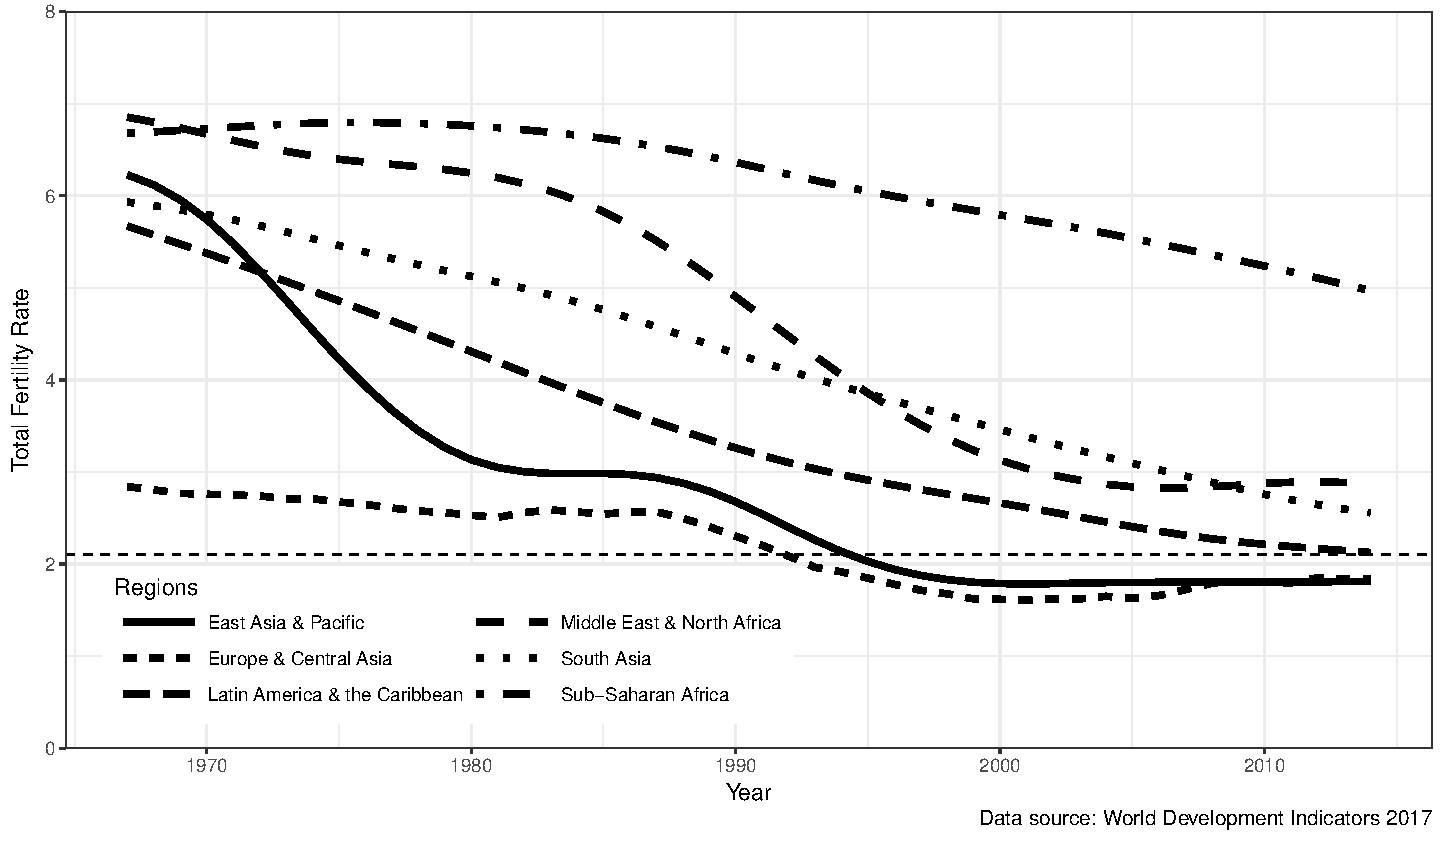
\includegraphics[width=0.95\linewidth]{../figures/totalFertilityRatesBW.pdf}
    \label{fig:TFR}
\end{figure}

If fertility levels in developing countries are quickly approaching
those of developed countries and there is rapid urbanization and
increasing labor force participation among women, does this Handbook
even need a chapter focused on fertility in developing countries? 
The goal of this chapter is to highlight areas in which a separate focus on
developing countries is still relevant, what the recent developments in
research have been, and most importantly, what I consider to be the main
outstanding issues. 
I begin with the question of why the changes in fertility behavior in
Sub-Saharan Africa's appear to be different from changes in other
developing countries. 
I then cover three areas where there are still likely to be substantial
differences between developed and developing countries. 
First, how couples time their fertility, and especially the interplay of
the timing of the first birth and educational attainment. 
Second, how differences in status and power in the household---what
economists refer to as bargaining power---affect fertility decisions. 
Third, the role in fertility decisions of the the strong preference for
boys over girls that still exist in many developing countries. 
The final part of the chapter reviews what we know about the effects of
different types of population policies in developing countries.

\section{Sub-Saharan Africa}\label{sub-saharan-africa}

Both in terms of the degree of decline and the overall level, the
outlier in Figure \ref{fig:TFR} is Sub-Saharan Africa. 
Sub-Saharan Africa now has an average TFR that is about twice as large
as in other regions. 
Most of the projected future increase in world population is therefore
likely to come from Sub-Saharan Africa \citep{Gerland2014}.%
\footnote{
Currently Africa is home to about 1 billion people, but this will
increase to between 3.1 and 5.7 billion by the end of the century at
current projected fertility rates.
} 
The most important issue from a policy standpoint is why the fertility
decline in Sub-Saharan Africa has declined at a much slower pace than
the other regions and even appears to have stalled in some countries
\citep{Ainsworth1996a,Singh2017}. 
The purpose of this section is not to provide the final answer, but
instead to highlight both how we can think about fertility decisions and
suggest possible answers. 
A caveat to the following discussion is that there are important
differences across countries within Sub-Saharan Africa that we cannot
cover in sufficient detail.

Broadly speaking there are two competing approaches to explaining
fertility decisions.%
\footnote{
This is clearly a simplification but it serves to illustrate the
differences in approaches.
} 
One sees fertility preferences as the main driver of fertility and
considers preferences malleable and mainly determined by cultural
factors and transmission of ideas of ideal family size across groups and
over time. 
Under this approach the main constraint to reaching desired fertility is
the level of access to family planning and contraceptives.%
\footnote{
See Adsera, this volume, for a discussion of fertility models as applied
to developed countries.
}

\begin{figure}[hp!]
    \centering
    \caption{Under-Five Mortality Rates by Region from 1967 to 2015 for Developing Countries}
    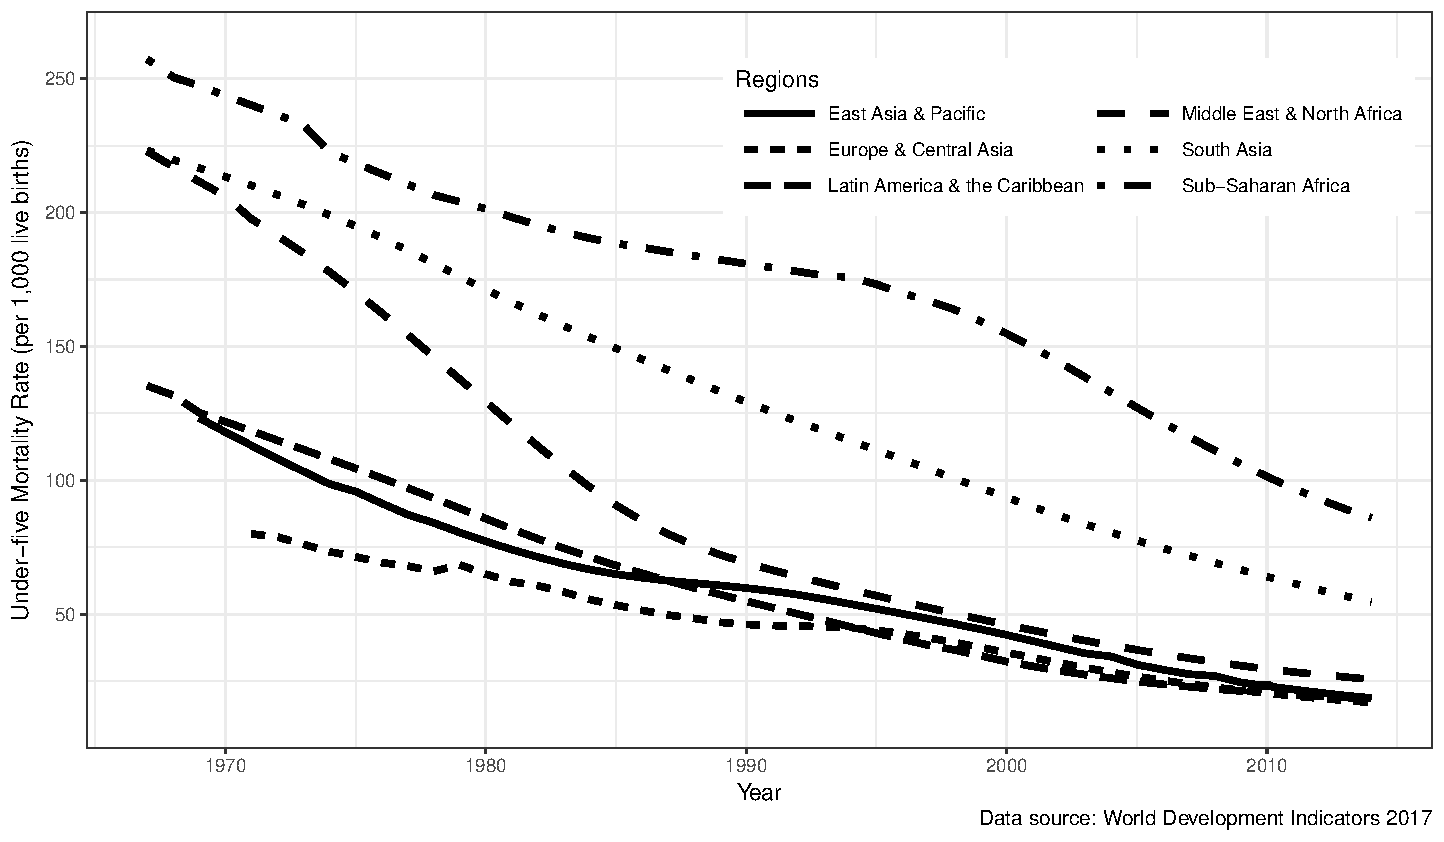
\includegraphics[width=0.95\linewidth]{../figures/childMortalityRatesBW.pdf}
    \label{fig:mortality}
\end{figure}

The other approach sees the fertility decision as driven by the
trade-off between the cost of children and the return to children, which
can either be monetary or the utility of having offspring. 
In this approach parents are assumed to be able to control fertility
even in the absence of modern contraceptives. 
Hence, although the lower cost of preventing births---for example easier
access to modern contraceptives---will still lower fertility in this
approach, the resulting decline in fertility is assumed to be much
smaller than in the first theory.

Both theories consider the surviving number of children as the main
outcome of interest. 
One possible explanation for the slow decline in fertility could
therefore be that mortality in Sub-Saharan Africa is higher than in the
other regions. 
Figure \ref{fig:mortality} shows the pattern in under-five mortality
rates across the same regions as above over time.%
\footnote{
The under-five mortality rate is the probability of dying between birth
and exactly five years of age, expressed per 1,000 live births.
}

The improvements in mortality risk over time are truly astonishing. 
Over the last half-decade the mortality of children under that age of
five in developing countries has fallen from close to 175 to below 50
per 1,000 live births. 
Sub-Saharan Africa, however, lags substantially behind other regions. 
Despite a massive improvement from a situation where more than a quarter
of all children born did not live to see their fifth birthday to about
80 deaths per 1,000 births, the current mortality rate is still more
than three times larger than that of the other regions (with the
exception of the Middle East and North Africa). 
Thus, although mortality is likely part of the explanation, it cannot 
be the full explanation. 
One way to see this is to compare fertility levels across regions when
they reach the same mortality level. 
For example, mortality in Sub-Saharan Africa is currently at the same
level as mortality was in South Asia around the turn of the century, but
fertility is about 1.5 children higher in Sub-Saharan Africa now than it
was in South Asia at the turn of the century.

If higher child mortality is not the explanation, what might lead to the
higher fertility in Sub-Saharan Africa? Demographers, following the
first approach described above, have argued that the two main reasons
for the slow decline in fertility in Sub-Saharan Africa are the high
ideal family size that is still in place and a substantial ``unmet
need'' for contraception
\citep{Bongaarts2013a,Casterline2017,Singh2017}. 
Contraceptive use is, indeed, lower in Sub-Saharan Africa than other
regions, but these other countries have managed to reduced fertility
even in the absence of access to modern contraceptives
\citet{Schultz1985,Galloway1987,Bailey1998,bengtsson06}. 
Furthermore, fertility in Sub-Saharan Africa has been---and still
is---characterized by longer birth intervals than in other regions even
in the absence of access to modern contraception
\citep{Caldwell1992,Moultrie2012,Casterline2016}. 
The longer birth intervals arise predominantly from longer postpartum
sexual abstinence and extended periods of breastfeeding compared to
other regions. 
To the extent that these behaviors are the result of conscious
decisions, the longer spacing suggests that people are able to control
fertility.%
\footnote{
It is still possible that fertility is higher than desired because the
higher cost of preventing ``accidental'' conceptions. 
This would explain why the estimated effect of access to family planning
in Ethiopia shows a reduction in fertility of about one birth, which is
equivalent to an approximate 20\% reduction in fertility
\citep{Portner2014a}.}

Three alternative explanations may explain the slow decline: the
relative abundance of land compared to other regions; low levels of
education or at least low levels of quality education; and the role of
urbanization across regions. 
Each of these is discussed in what follows.

There are two important characteristics of land access in Sub-Saharan
Africa that may explain the higher fertility rates in this region. 
First, there is, on average, more land per capita in Sub-Saharan Africa
than in the other regions. 
At the median projected population growth for Sub-Saharan Africa---which
is 4.2 billion people by 2100---the population density will only be
roughly equal to that of China today \citep[p 235]{Gerland2014}. 
The low density means that there is little pressure to restrain
fertility for fear of running out of land. 
In fact, it is likely that there is a higher return to children in
Sub-Saharan Africa than in the other regions---or, at least, a
substantially lower cost---because the return to children working on the
family farm is higher \citep{Caldwell1992,Bongaarts2013a}. 
Similarly, there are substantially higher return to having wives work on
agricultural land \citep{jacoby95,Matz2016}. 
The associated polygyny in some countries also appeared to have resulted
in a situation where the cost of the children is borne by the individual
wives, but the decision regarding fertility iss made by the husband. 
I return below to how husband and wife decide on fertility if they do
not have the same desired number of children.

A second characteristics of land in Sub-Saharan Africa that also can
lead to higher fertility is that---despite its abundance---access to
land rights are in many countries controlled at the local level by
chiefs and other local institutions rather than through market-based
buying and selling of land. 
This is important because the main method used to maintain the
productivity of agricultural land is often through fallowing, and with
less secure land rights farmers may fallow their land for shorter
periods than those with more secure rights \citep{Goldstein2008}.%
\footnote{
See also \citet{besley95c}, who discuss other investments in land that
can secure property rights.} 
The reason a lack of secure land rights can lead to higher birthrates is
that land is often allocated based on the number of household members. 
Hence, more children, everything else equal, increases a household's
claim to land access. 
The irony here is, of course, that if everybody else follows the same
strategy, the result will be much higher fertility and little change in
the allocation of land.

For both of these potential effects of land access on fertility we,
however, have little direct information on their effects, and the role
of land in fertility is one area that calls out for future research. 
This is, however, made more difficult by the need to measure land
access. 
Although we obviously have information on total land area for countries,
measuring arable land is often more difficult, complicating efforts to
compare land access and fertility across countries. 
At the individual level we would need information on and exogenous
variation in \emph{potential} land access---that is, how much land
parents expect to have access to for a given number of children---and as
the second argument shows land allocation is not a random process. 
Specifically, if there are unobserved characteristics that influence
both how much land parents have access to and their number of children,
the relationship between current land access and number of children will
provide a biased estimate of the effect of land access. 
One approach would be to use \emph{de jure} or \emph{de facto} changes
in land laws or programs aimed at securing land rights for farmers and
examine their effects on fertility.

So far, there are only a few examples of this approach in the literature.
An early example is \citep{de_vany77} using data from Mexico.
Although they were mainly interested in the fertility increasing effects 
of uncertainty in genearl, their results indicate that providing more 
\emph{secure} land access by moving away from Mexico's ejido system---where 
land is collectively owned and distributed partly according to family 
size---to a market based system would lower fertility.
More recently, \citep{Ali2015} examined a case where the southern part of
the Amhara region in Ethiopia abolished the historic system where land 
was distributed based on family size, but the northern did not.
Because fertility in the two parts of the region would arguably have 
developed the same in the absence of this change, the differences over
time and across areas can be used to identify the effects of the
policy change.%
\footnote{
This is known as a difference-in-difference approach because you
take the difference between how the two areas' fertility changes
over time.
}
Moving away from the pro-natalistic land distribution system is
estimated to reduce fertility by just over one child for rural 
households.
These results suggests that security of land access is important, 
although none of them can directly address whether the higher fertility
in Sub-Saharan Africa is driven by an abundance of land.


A second potential explanation is differences in the effect of education 
on fertility. 
The standard economic model of fertility considers the opportunity cost
of women's time to be the main factor affecting the number of children;
as the cost of women's time increases with more education fertility 
falls in response \citep{becker91}. 
There is a large literature documenting a substantial negative association 
between women's education and fertility \citep{strauss95}.
Higher education is also associated with better health outcomes for both 
women and children.
This is relevant because better health outcomes lead to lower child 
mortality, which, in turn, further decreases fertility, because fewer 
births are required to reach a desired number of surviving children 
\citep{Ainsworth1996}. 
The strong association between higher maternal education and lower fertility 
is essentially universal, making it the main recommended way to decrease 
fertility \citep{schultz02}.
There is less causal evidence on the effects of education on fertility
and health, although what we have supports the idea that higher education
leads to lower fertility and better health 
\citep{Breierova2004,Behrman2015,Keats2016,Ozier2016}.%
\footnote{
It is not completely clear exactly why there is such a strong
effect of education on child health.
\citet{Thomas1991}, \citet{Glewwe1999}, and \citet{Kovsted2002}
all suggests that it is better knowledge about health rather 
than higher income, changes in norms, or something inherent in 
education that drives the postive relationship between education
and health.
} 

Fertility, however, begins to decline at higher levels of education in
Sub-Saharan Africa than in other regions and the relationship between
fertility and education may even be positive for low levels of education
\citep{Ainsworth1996,Benefo1996,Thomas1996}. 
Part of the problem may be the quality of education in Sub-Saharan
Africa. 
In other words, the stated number of years of education may be a worse
predictor of actual human capital accumulation in Sub-Saharan Africa
than other regions.%
\footnote{
As shown by \citet{Oye2016} this is not the same as saying that low
quality education has no impact on fertility; only that the effect of
education on fertility is lower the lower the quality of the education
received.}

A good example of this problem is Tanzania
\citep{Galabawa2001,Wedgwood2005}. 
Taken at face value, Tanzania has a very high reported education level. 
This is most likely the result of the 1974 Universal Primary Education
Movement, which increased accessibility of primary education and
enrollment rates. 
The problem is that the quality of education reportedly was very low. 
In addition, the economic crisis Tanzania experienced in the 1980s
further lowered the quality and enrollments declined significantly. 
Hence, it is unclear to what extent reported education levels reflect
women's actual human capital. 
The result is that education does not appear to have as substantial an
effect on fertility in Tanzania as other found elsewhere
\citep{Alam2016}.

The final potential explanation for differences in TFRs across regions
is the role of urbanization. 
One topic that seems to be essentially absent in discussions about
fertility and its determinants in Sub-Saharan Africa is the difference
between urban and rural areas. 
As a rule, all regions have had and still have higher fertility in rural
areas than in urban areas. 
This is directly in line with what we expect. 
The cost of children is clearly higher in urban areas than in rural
areas, even for women with the same amount of education---and therefore
the same opportunity cost of time. 
Sub-Saharan Africa is no different. 
An example is Ethiopia in 2011, where the overall TRF is 4.8, but that
masks a TFR of 5.5 in rural areas and only 2.6 in urban areas
\citep{Central-Statistical-Agency/Ethiopia2012}. 
Part of the explanation for the lower fertility is the higher average
education level of women in urban areas than in rural areas. 
But, even for women with the same education level, fertility is lower in
urban areas than in rural areas \citep{Ainsworth1996}.

There has, however, not been a systematic examination of how fertility
varies with education in urban areas across different regions. 
If predicted fertility is similar across regions for the same level of
education, that would suggest that Sub-Saharan Africa is not inherently
different. 
A lower ``return'' to education could either be an indication that the
quality of education is lower, that the opportunity cost increases with
higher education is not as high in Sub-Saharan Africa as in other areas
(either because of the lower quality or because of lower levels of
development), or it could suggest that there is something inherently
different in what determines fertility in Sub-Saharan Africa than in
other regions.

\section{Timing of Fertility}\label{timing-of-fertility}

How couples decide on when to have their children is relevant both
because it provides us with an idea of how good people are at
controlling their fertility and because timing of births may impact the
health of both a mother and her children.%
\footnote{
The idea that people plan their fertility is not without opposition. 
\citet{Timaeus2008} and \citet{Moultrie2012}, for example, argue that
``postponement'' of births---that is, simply not having a birth now---is
different from decisions on the spacing between births and the overall
number desired.} 
We know, however, surprisingly little about what determines the timing
of births in developing countries. 
With increasing numbers of women entering the labor force in developing
countries, understanding how timing decisions are made will be important
for the design of suitable policies. 
The lack of research is partly because of data limitations and partly
because of the difficulty in identifying the causal relationship between
timing and other decisions, such as labor supply. 
The two sub-areas where we do have some information are the timing of
first births and how the sex of the last child affects timing of the
next birth. 
This section covers the timing of first birth and leaves the other for
the sections below on sex preference.

Having a first birth earlier in life is associated with lower
educational attainment, higher completed fertility, and worse health and
labor-market outcomes.%
\footnote{
See also the discussion of the literature on the association between
short birth spacing and child health more generally in
\citet{Casterline2016}.} 
This is, however, not necessarily indicative of a causal relationship
between earlier first birth and the other outcomes. 
A woman who, for example, has a lower expected return to education may
decide that using contraceptives is not worth the cost and therefore
would be more likely to conceive and subsequently drop out of school. 
Furthermore, as long as fertility is well below natural fertility
levels, having an earlier birth will not, in itself, increase total
fertility.%
\footnote{
Natural fertility is the level of fertility that would prevail in a
population that makes no conscious effort to limit, regulate, or control
fertility.}

For this reason, most of the literature has focused mainly on what
determines the timing of first births and, to some extent, on whether
women are more likely to drop out of school after their first birth. 
In the relatively small literature on timing of first births, there are
two main approaches to trying to identify a causal relationship between
timing of first birth and other outcomes. 
One is to look for variables that plausibly only affect one or the
other, with no direct effect on the other outcomes, and then jointly
estimate the various decisions.%
\footnote{
This approach is often combined with restrictions on the correlation of
error terms across decisions.} 
The other approach is experimental, where researchers randomly grant
access to a program that is believe to influence one of these decisions
and then examine whether the timing of births and the other outcomes are
affected by the program. 
Independent of method, the results suggest that increasing education is
important in delaying marriage and first birth
\citep{Duflo2015,Marchetta2016}.

The downside of both approaches is that we cannot learn much about what
completed fertility is going to look like. 
Even experiments that follow people for an extended period, like the
seven years in \citet{Duflo2015}, only extends to the beginning of the
prime childbearing years, ages 20 to 30. 
An important caveat is also that the effects of interventions may
disappear quickly after the end of the program \citep{Baird2016}.

\section{Bargaining Power}\label{bargaining-power}

An important question is what happens when husband and wife do not agree
on the desired number of children. 
The original literature on this question mainly showed that families do
not necessarily behave as if husband and wife have similar preferences. 
One way to see this is to look at unearned income---mainly income that
does not come from the application of skills and labor---that can be
attributed to either the wife or the husband. 
If the number of children born changes with shifts in the distribution
of this income, this indicates that the partners have different
preferences.

Results from Thailand as of the 1980s show that women with more
``bargaining power'' spent less time working and preferred to have more
children \citep{Schultz1990}. 
The result that women prefer more children is not generally supported,
however, and in most cases men have a higher preferred number of
children than women \citep{Westoff2010}. 
An example of this is Malaysia where both ethnic Chinese and ethnic
Malay husbands had a higher ideal number of children than their wives,
although the ideal numbers were below the actual number of children for
both partners \citep{Rasul2008}.

Sub-Saharan Africa is often considered a special case when it comes to
different preferences for the ideal number of children across husband
and wife. 
The father bears less of the cost of children than in other developing
countries because of the family structure.
This is especially the case in West Africa where husband and wife often 
make separate economic decisions and may not even share the same house,
and where polygyny is more prevalent 
\citep{Caldwell1992,Udry1996,Tertilt2005}. 

It would seem that in cases like this, it would be beneficial to provide
women with more control over use of contraceptives. 
An experiment in Zambia tried exactly that \citep{Ashraf2014}. 
One group of women was given an individual voucher for free and
immediate access to contraceptives. 
Because the most popular contraceptives are injectables, they were able
to hide contraceptive use from their partners if they wanted to. 
In the other group, husbands were given the vouchers and both the
husband's and wife's signatures were required to redeem it. 
As expected, the women who needed their husband's signature were less
likely to visit a family planning nurse and less likely to use
injectable contraceptives. 
As a result, these women were also more likely to have a birth. 
The caveat is that women who could potentially conceal their use of
contraceptives reported significant reductions in happiness, health, and
ease of mind, compared to the women in the group where both signatures
were required.

When discussing differences in preferred number of children across men
and women it is important to realize that in some countries men do end
up with more children than women \citep{Field2016}. 
Using data from eight Sub-Saharan African countries, men have, on
average, more children than women of the same cohort in seven out of the
eight countries. 
The gaps are large, ranging from 0.8 children in Zambia to 4.6 children
in Burkina Faso, but appear to be decreasing over time. 
This pattern is consistent with men partnering with younger women in a
situation where the population is growing and also with polygyny. 
This indicates that that differences in desired number of children are
often mirrored in differences in actual achieved fertility. 
The implication is that there might not be an innate contradiction
surrounding fertility behavior within couples, at least in countries
with growing populations \citep{Field2016}.

\section{Sex Preference}\label{sex-preference}

An especially important aspect of intrahousehold allocation is the
preference for children of a specific sex.%
\footnote{
Rose, this volume, reviews the literature on child gender in developing
and developed countries and discusses methodological issues that arise
when studying child gender effects} The dominant version is a strong
preference for sons in many countries, most notably in India and China. 
The literature is somewhat fuzzy on what exactly constitutes son
preference. 
One popular version is that for their ideal number of children, parents
would prefer to have more sons than daughters, and the strength of son
preference is then measured by how many more sons than daughters a
family wants.%
\footnote{
In India's National Family Health Surveys conducted, in and Demographic
and Health Surveys in general, son preference is measured as part of the
general fertility questions. 
The first question is how many children a woman would have if she could
choose exactly how many. 
This if followed by the sex preference question: ``How many of these
children would you like to be boys, how many would you like to be girls
and for how many would the sex not matter?''} This measure of son
preference is commonly used in the literature
\citep[e.g.]{clark00,Jensen2009,Hu2015}. 
Other versions are possible. 
Parents might, for example, have a preference for one son, but once that
one son is secured they do not have strong preferences for the
distribution between sons and daughters for the remaining children.

Before prenatal sex determination became available, most research
focused on the impact of son preference on fertility decisions and
spacing between births. 
This literature showed clearly that in areas with son-preference,
families were more likely to stop childbearing after the birth of a son
than after the birth of a daughter \citep[see, for
example,][]{Das1987,Arnold1997,clark00,filmer09}. 
Furthermore, in the absence of sex-selective abortions, son-preference
often leads to a shorter birth interval if the previous birth was a
daughter \citep[see, for
example,][]{Das1987,Rahman1993,Pong1994,Haughton1996,Arnold1997}. 
The resulting shorter spacing is a possible explanation for worse health
outcomes for girls
\citep{arnold98,Whitworth2002,Rutstein2005,Conde-Agudelo2006}. 
There is also evidence that girls were underreported in China as a result
of strong son preference combined with the one-child policy
\citep{Merli2000,Goodkind2011}.

With the introduction of amniocentesis, ultrasound, and chorionic villus
sampling (CVS), it became possible to tell the sex of a fetus and abort
the pregnancy if the fetus was not of the preferred sex. 
By itself, this may not have led to substantial changes, but combined
with lower desired fertility as in India or forced lower fertility as in
China, the availability of prenatal sex determination had substantial
impacts on the sex ratio. 
It is easy to see how declining fertility can increase the use of sex
selection. 
Consider a family that wants one son. 
If the family is willing to have up to 4 children, the probability of
having a son is more than 94 percent, even without sex selection, and
that increases to almost 99 percent if the family is willing to have up
to 6 children.%
\footnote{
The probabilities of not having a son are 48.8 percent for one child,
23.8 percent for two children, 11.6 percent for 3 children, 5.7 percent
for 4 children, 2.8 percent for 5 children, and 1.4 percent for 6
children.} 
If the desire is instead for one son \emph{and} a maximum of two
children, there is a 24 percent chance that the family will have to
resort to sex selection to achieve both targets.

There is relatively little empirical analysis of the effects of
fertility on sex selection using individual-level data
\citep{park95,Ebenstein2011}. 
At the country level \citet{Bongaarts2013} shows how sex ratios at birth
are only elevated for countries with lower fertility and
\citet{Bongaarts2015} use national-level estimates of the relationship
between the sex ratio at birth and fertility as part of their prediction
of the number of missing women past and present. 
Furthermore, simulations suggest that in Korea the introduction of sex
selection changed family size little, but did result in abortions of
female fetuses equal to about 5 percent of actual female births
\citep{park95}. 
For China allowing a three-child policy has been predicted to increase
the fertility rate by 35 percent, but also reduce the number of girls
aborted by 56 percent \citep{Ebenstein2011}.%
\footnote{
Strong son preference does not, however, automatically lead to high use
of sex selection. 
One example of this is Turkey \citep{Altindag2016}
}

Research suggests that son preference in India, when measured as ideally
having more boys than girls, decreases both over time and with higher
education and wealth \citep{bhat03,pande07,Gaudin2011}. 
This may, however, be an artifact of the retrospective nature of the way
desired fertility questions are often asked. 
If parents were instead asked about the desired sex composition for a
specific number of children, the results are different
\citep{Jayachandran2017}.%
\footnote{
Parents were asked about their desired sex composition for their
children's children to avoid the retrospective nature of the standard
sex preference questions. 
The question was: ``Suppose your son/daughter [the specific grade 6 or
7 child we surveyed]
was going to have $N$ children. 
How many of them would you want to be boys and how many would you want
to be girls?'' The $N$ was a randomly chosen number between one and
five.} 
The lower the given number of children, the higher the proportion of
boys to girls was. 
This result is consistent with evidence that women with more education
and urban women are more likely to use sex selection
\citep{Portner2015b}. 
These women have higher costs of children and therefore lower desired
fertility.

\section{Policies}\label{policies}

Even though most people automatically think of family planning programs
when population policy in developing countries is mentioned, any policy
that changes the opportunity cost of time or affects the distribution of
bargaining power within the household will also affect fertility. 
Therefore both standard family planning programs and other policies that
impact fertility are discussed in this section.

Despite a substantial and long-standing interest in the effectiveness of
family planning programs, there is relatively little convincing
empirical evidence.%
\footnote{
For a more in-depth discussion of both the history of family planning
programs and the literature, see \citet{Miller2016}. 
An older review of the literature, focusing on whether access to family
planning changes preferences for number of children, is in
\citet{Freedman1997}. 
\citet{Singh2012} provide recent estimates of the use and need for
contraceptives in the developing world, together with cost of providing
contraceptive services.} 
The lack of evidence is mainly the result of the challenges in measuring
family planning program's impacts. 
First, studies of family planning programs have often occurred during
periods of rapid economic development and fertility decline, making it
difficult to isolate the effects of family planning programs from the
changes in the economy. 
Second, existing studies have largely ignored heterogeneous impacts,
specifically whether women with different education levels respond
differently to family planning. 
Evidence from the US indicates that better-educated women and
less-educated women are equally efficient users of modern
contraceptives, but better-educated women are more efficient at using
``ineffective'' contraceptive methods such as withdrawal or rhythm
\citep{Rosenzweig1989}.%
\footnote{
This is supported by the differences in the effect of the roll-back of
abortion access in Romania, which resulted in bigger increases in
fertility for less-educated women than better-educated women
\citep{Pop-Eleches2010}.} 
This suggests that the effect of family planning should be stronger, the
lower the education levels, but few studies address this for developing
countries.

Finally, rigorous study is hampered by the challenge of non-random
program placement \citep{rosenzweig86,pitt93,Miller2016}. 
For example, unobserved characteristics of both women and the areas they
live in might lead some women to be more likely to both have access to
family planning and to use it. 
In that case, simply looking at the correlation between use of family
planning and fertility will overstate the strength of the relationship
in the general population.

Randomizing the allocation of programs and comparing the outcomes of
interest between treatment and control areas would seem to overcome the
non-random program placement problem. 
Although theoretically superior, such experiments have several drawbacks
in practice \citep{Portner2011}. 
First, the experiments are often small in scale, which makes it more 
difficult to establish whether an effect exists (what is known as low
power).
Second, non-compliance of randomization can further decrease the
power of the experiment. 
This is particularly a problem for family planning programs where
the randomization takes places at the community level and where it
is harder to avoid spill-over of, for example, information about 
contraceptives to non-treatment areas. 
Finally, because of the cumulative nature of fertility, an experiment
must run for a substantial period before one can assess the effect on
fertility. 
The absence of an increase in contraceptive use from an experiment 
in Ethiopia is, for example, likely because of the experiment's 
short duration \citep{Desai2011}. 
When run for too short a period, experiments may also be more prone to
adverse effects of unanticipated short-term problems.
One example is the health scare experienced by an experiment
in Zambia, where people were led to believe that injectable
contraceptives contained HIV resulting in a four months national ban
and a very small effect on fertility \citep{Ashraf2009}.%
\footnote{
The published version of this paper, \citet{Ashraf2014}, does not 
mention the scare.}
Even if an effect is found, these short-run effects may simply reflect
changes in spacing-patterns rather than changes in the overall number of
children. 

The Matlab family planning program from Bangladesh is the least likely
to suffer from these drawbacks. 
It began in 1978, when the International Centre for Diarrhoeal Disease
Research, Bangladesh (icddr,b) introduced a family planning program in
70 of the 149 villages covered by the demographic surveillance system in
the area. 
The icddr,b family planning program was characterized by an outreach
program, consisting of home visits by trained female outreach workers. 
By 1984, fertility was 24 percent lower in the villages that received
the intensive family planning program compared to the villages that
received only the standard family planning program \citep{Phillips1988}.

More recent work using the same villages with data until 1996 finds a
decline in fertility of about 15 percent in the program villages
compared with the control villages, despite rapid declines in fertility
in the control villages \citep{Sinha2005,Joshi2007}. 
These results reflect, however, a level of program intervention and
intensity that some argue are unlikely to be sustainable
\citep{pritchett94a}.%
\footnote{
Per woman reached, the program cost 35 times more than the standard
government family planning program and each averted birth cost \$180 in
1987, 1.2 times GDP per capita at the time.} 
Using a quasi-experimental approach, the Navrongo Project in northern
Ghana also found an initial 15 percent reduction, although that was
based only on the initial 3 years of the program \citep{Debpuur2002}. 
There is no evidence of a long-run effect of the project on fertility
after 15 years \citep{Phillips2012}.

If longitudinal data were collected in parallel with the introduction of
the program, program effects can be estimated using fixed effects,
provided there are enough areas that receive a program between the
(minimum) two survey rounds and provided the period between the rounds
is long enough. 
Examples from Indonesia of this approach found a negative (but not
statistically significant) effect on fertility, responsible for only 4
to 8 percent of the decline in fertility from 1982 to 1987
\citep{pitt93,Gertler1994}. 
Longitudinal data are, however, most often not available or cover only
short periods, in practice limiting researchers to using cross-sectional
data.%
\footnote{
There are also additional problems with using fixed effects, such as
measurement error bias. 
For a discussion of this and other problems in the study of family
planning see, for example, \cite{angeles98}.}

If neither experiments nor longitudinal data are available, an
alternative approach is to use variables that influence program
placement but are unrelated to individual fertility, what is known as
the instrumental variable (IV) approach. 
This is the least appealing approach when trying to identify the causal
impact of family planning because it relies heavily on the choice of
variables that affect program placement without any direct test for
whether these variables are appropriate. 
Despite these drawbacks, it is often the best that can be done to
address endogeneity concerns given the constraints.

Using this approach, a woman in Tanzania exposed to family planning
throughout her fertile lifespan is found to have 4.13 children compared
with 4.71 children in the absence of family planning programs
\citep{angeles98}.%
\footnote{
See also \citet{Angeles2005} on Indonesia and \citep{Angeles2005a} on
Peru.} 
Lingering concerns remain, however, that some of the instruments used to
identify placement (such as child mortality levels and the presence of
other family planning services) may also be correlated with unobservable
variables that influence both placement and fertility decisions. 
Examining the difference in effects of providing subsidies for
contraceptives or expanding access to previously not served areas,
results from Indonesia show that subsidizing contraceptive by about half
of the total cost lowers fertility by about 3 to 6 percent, whereas
expanding the distribution network by one standard deviation lowers
fertility by about 12 percent \citep{Molyneaux2000}. 
These results are consistent with what is found for Profamilia,
Columbia's family planning program, which reduced lifetime fertility by
around half a child, equivalent to less than 10 percent of the sharp
decline in fertility over the period the program was implemented
\citep{Miller2010}.

While most studies find an effect of about half a child,
\citet{Portner2011} find a substantially larger effect of access to
family planning in Ethiopia.%
\footnote{
The half a child reduction is also found in Romania using that country's
ban on abortion and other birth control, with bigger effects the less
educated the woman \citep{Pop-Eleches2010}.} 
Access to family planning reduces completed fertility by more than 1
child among women without education, which is equivalent to a 20-25
percent reduction. 
No effect is found among women with some formal schooling, suggesting
that family planning and formal education act as substitutes, at least
in this low income, low growth setting.%
\footnote{
These results run counter to the argument in \citet{Feyisetan1996} that
low education is a constraining factor in the uptake of contraception,
although their data cover a period before long-acting injectable
contraceptives became widely available. 
There is mixed evidence from the Matlab family planning program on
whether the program acted as a substitute for female education in the
reduction of fertility \citep{Sinha2005,Joshi2007}.
} 
This highlights the importance of examining how access to family
planning can vary depending on the recipients' characteristics.

A very different approach to understanding how family planning access
affects fertility is to examine the response to disruptions in access or
substantial changes in the price of contraception. 
These are---by their very nature---often temporary and therefore cannot
tell us much about final fertility outcomes, but they do have the
advantage here of mostly being exogenous to the individual women. 
That is, the disruption in supply of contraceptives comes as a surprise
and is independent of the individual women's initial demand for
contraception.

The 1997 financial crisis in Indonesia led to very large changes in
prices of contraceptives, because it reduced the government's ability to
subsidize the price of contraceptives \citep{McKelvey2012}. 
Despite the large price changes there were few changes in either the
choice of method or the decision to use contraceptives. 
This result holds even for the poorest couples who are most likely to
rely on the subsidy for access to contraceptives.

The United States' implementation of the Mexico City Policy%
\footnote{
Also often referred to as the ``Global Gag Rule''. 
It was originally implemented in 1984 under the Reagan administration, 
rescinded during Clinton, then reinstated again under Bush, and 
rescinded under Obama.
The Trump administration went even further than the original 
implementations and the policy now applies to all global health
assistance.
}, which forbid funding non-governmental organizations (NGOs) that perform
or promote abortion services, has also been used to identify the effects
of access to contraceptives because most of the NGOs affected also
provide subsidized contraceptives. 
In Ghana, contraception availability and use were reduced during the
periods the policy was in effect \citep{Jones2015}. 
This led to significant increases in conception for rural women, but not
for urban women. 
Within rural areas, the poorest women were the most affected with a 7 to
10 percent higher fertility, whereas less poor women saw increases of 3
to 6 percent. 
Perversely for a policy aimed at reducing abortions the effect was
exactly the opposite. 
Rural Ghanaian women in the upper three wealth quintiles aborted 4 out
of every 10 additional pregnancies that were the result of the lower
contraception availability. 
The poorest women did not change their abortion behavior and therefore
ended up with significantly more children.

That the policy increases the use of abortions is supported by analyses
of cross-country data for Sub-Saharan Africa \citep{Bendavid2011}. 
Using data from 1994 to 2008, countries were divided into ``high
exposure'' and ``low exposure'' countries, depending on the level of
financial assistance per capita provided by the United States when the
policy was not active. 
The probability of having an abortion for a woman in a ``high exposure''
country was more than twice that of a woman in a ``low exposure''
country when the policy was in effect. 
Furthermore, there was no apparent difference in abortion rates when the
policy was not in effect and the abortion rate in ``high exposure''
countries began to rise only after the policy was reinstated in 2001. 
Finally, the use of modern contraceptives stopped increasing after 2001
in ``high exposure'' countries, whereas ``low exposure'' countries
continued to see increases in contraception use.

A different type of supply interruption is found in the Philippines,
where a scheduled phase-out of international donations of contraceptives
combined with decentralization of the responsibility of providing
contraceptives and supply chain issues resulted in substantial variation
in the availability of contraceptives over time and across area
\citep{Salas2014}. 
Both supply reductions and swings in the supply of contraceptives lead
to significant increases in the number of births. 
The poorest women, those living in rural areas, and those with less than
a high school education, were the most affected by supply fluctuations. 
The Philippines were also the location of an outright ban on modern
contraception in the city of Manila. 
Comparing Manila and other cities in the capital region, and assuming
that these cities would have had similar fertility trends in the absence
of the ban, the ban resulted in an approximately 3 percent increase in
the number of children \citep{Dumas2017}. 
This effect is larger, the younger the mother.

Probably the most well-known and strictist approach to population
control is China's one-child policy, which began in 1979.%
\footnote{
\citet{Byker2012} analyze the effects of the aggressive use of
sterilization, which reported involved bribes and coercion, initiated by
President Fujimori of Peru.} 
Households that exceeded their ``birth quota'' were penalized, but the
birth quota depended on ethnicity and later on the sex of the first-born
child \citep{Li2005}.%
\footnote{
Ethic minority women were allowed two children until the late 1980s.} 
Furthermore, there was substantial heterogeneity in how the policy was
implemented across regions. 
Women in urban areas who exceed their birth quota were, for example,
generally punished much more severely than women in rural areas.

Despite the scale of the program, there has been little research
directly on the effects of China's one-child policy on fertility. 
Part of the problem is access to reliable data, as is often the case for
China, and another problem is that since this is a national policy
everybody should, in principle, be affected equally. 
One study, however, used differences in the implementation of the policy
across areas and found an 11 percent reduction in the probability of a
second birth; the policy was more effective among urban and
well-educated women \citep{Li2005}.
Interestingly, the policy had almost no effect on the least well-off
group, which consists of rural residents with little or no education. 
To the extent that having fewer children translates into better health
and education outcomes for children as suggested by \citet{becker73},
this disparity in the effect may lead to increased inequality.%
\footnote{
Although, \citet{Rosenzweig2009} find only small increases in education
investments as a result of the policy and its associated decline in
fertility.}
A similar approach using differences over time and across areas in the 
fines levied on couples that do not adhere to the policy also shows
that the policy substantially lowered fertility \citep{Ebenstein2010}.%
\footnote{
This reduction in fertility is also associated with a substantially
higher male-to-female sex ratio, presumably because of increased use
of sex selection. 
}

Whether or not family planning programs have a substantial effect on
fertility, it is possible that they can improve the well-being of both
women and children simply through providing better control over the
timing of births. 
Despite assertions such as ``{[}w{]}hat is hardly in dispute is the
association between inter-birth intervals and health outcomes for mother
and child, in particular the deleterious impact of short intervals.''
\citep[p. 
175]{Casterline2016}, there is even less solid research on the effects
on other outcomes than there is for the effects on fertility. 
The main problem is that identifying the causal effect of
family-planning programs is particularly difficult for outcomes other
than fertility, because a woman's fertility and other outcomes such as
her health and her investment in her children are likely driven by the
same unobserved characteristics and the decisions are jointly made
\citep{Schultz2005}. 
A woman may, for example, end up with a short duration between two
births because she has low bargaining power, and the low bargaining
power may also mean that she is less likely to receive health care. 
In that case, the cause of a poor health outcome is not necessarily the
short birth spacing, but the underlying problem of her low bargaining
power. 
In addition, many of the outcomes of interest, such as children's
completed education, will not be known until many years later.

The Matlab experiments described above contribute most of the credible
research in this area, exactly because they provide a random assignment
of family planning and thereby avoid the problem of unobserved variables
affecting both fertility and other outcomes. 
Despite the substantial reduction in fertility that followed from the
differential access to family planning, there is little evidence of
significant effects on the school enrollments of boys or girls
\citep{Sinha2005}. 
Using a slightly different sample, there is some evidence that younger
boys completed more schooling with access to the program, but the effect
is smaller for older children, and not statistically significant for
girls of any age \citep{Joshi2007}. 
The effect of the program on labor force participation is positive for
both boys and girls, but only significant for boys. 
Furthermore, the effect of the program on our most common measure of
health, the height of children, is unclear, with some research
suggesting no significant differences in height for children less than
15 years old across treatment and control areas \citep{Joshi2007} and
other finding a significant effect \citep{Barham2012}.

Even though the results on education and health are mixed, children in
the Matlab treatment areas are significantly more likely to survive
\citep{Joshi2007}. 
Having access to the program reduced under-five child mortality by five
percentage points. 
In addition, preventive health inputs were used more frequently in the
treatment areas, as are prenatal care and tetanus inoculations for
mothers. 
The substantial decline in child mortality point to substantial
improvements in early child health as a result of the program.

For adults, there is substantial evidence that women benefit from access
to the program \citep{Joshi2007}. 
Women in the treatment areas had substantially higher BMI, which is
correlated with better health in a malnourished population like the one
in Matlab. 
They were also more likely to have access to drinking and
cleaning/bathing water sources within the family compound. 
Furthermore, some effects of the program vary by education level.
Treated women with more education at the beginning of program were
more likely to live in higher-valued homesteads, own more agriculture,  
nonagricultural and financial assets, and earned larger market incomes
compared to similarly educated women in the non-treatment areas.
For low education women there is no significant difference in these
outcomes between treatment and control areas.

One argument for why we sometimes fail to find substantial changes in
fertility from access to family planning is that many people in
developing countries had little incentive to reduce the number of
children; the opportunity cost of women's time is low and children are
potentially productive on the family farm or can serve as old age
security \citep{Banerjee2014,Lambert2016}. 
As a result, rather than focusing on the supply of family planning, some
economists emphasize policies that influence fertility demand, such as
household poverty and girls' schooling
\citep{pritchett94a,DasGupta2011}.

The most important of these policies is women's schooling \citep{schultz02}. 
The basic idea is that children require both parents' time and goods and
these inputs combine to produce a child and its traits. 
The most costly input is the mother's time. 
Not only does pregnancy take its toll on the mother's productivity in
the labor market, children also require a substantial amount of time
after they are born and until they are able to fend for themselves. 
With increasing education come increases in wages and productivity. 
Hence, as women receive more education their (potential) wage increases,
which means that the opportunity cost of their time also increases. 
In other words, the more education the mother has the higher is the cost
of having children in terms of foregone income. 

Furthermore, even the perception of an increased opportunity cost lead
to a postponement of marriage and fertility and lower desired fertility.
A particularly nice demonstration of this comes from an experiment in India, 
which randomly selected rural villages to inform about the potential for women
to work in the emerging business process outsourcing industry \citep{Jensen2012}.
The rapid growth of this industry led to a sharp increase in the demand
for educated female workers but awareness of the opportunities were limited.
In villages that were provided with information about the job opportunities
there were an increased in human capital investments for girls and
delayed marriage and childbearing for women. 
Women in the treated villages also report wanting to work more and have 
fewer children in their lifetimes.

The increase in the opportunity cost of children for mothers with more
education is not the only potential explanation for why education is
associated with lower fertility. 
Higher education of women is also associated with significantly better
child health, although it is unclear exactly what leads to this
association.
\citet{Thomas1991}, \citet{Glewwe1999}, and \citet{Kovsted2002}
all suggest that it is better knowledge about health rather 
than higher income, changes in norms, or something inherent in 
education that drives this postive relationship between education
and health.
No matter the reason, better health outcomes for children allow women 
to achieve their preferred number of children with fewer births. 
In addition, more education may lead to a better bargaining position for
women and if women prefer to have fewer children than men this would
reduce fertility.%
\footnote{
\citet{Ainsworth1996} reviews other potential explanations.}

\section{Conclusion}\label{conclusion}

As this article has shown, most developing countries have experienced a
substantial decline in fertility over time. 
In fact, most countries are now getting close to replacement level. 
This does not, however, mean an immediate stop in population growth
because of the large number of young people who have still not entered
reproductive age in many countries. 
Furthermore, Sub-Saharan Africa has not experienced as strong as decline
in fertility and in some cases the decline has stalled. 
I suggest three possible explanations may explain why Sub-Saharan
Africa's fertility experience is different: a relative abundance of
land, the lower quality of education, and urbanization. 
Understanding fertility in Sub-Saharan Africa is clearly an area that
deserves further research.

In addition to fertility behavior in Sub-Saharan Africa, there are three
important areas where we have limited knowledge when it comes to
fertility decisions in developing countries. 
First, what factors determine the timing of fertility, especially for
first births, and the relationship of birth timing to schooling and
labor market outcomes? Second, what is the role of bargaining power when
determining fertility? Finally, how do sex preferences affect fertility
outcomes? Common to all of these is the difficulty in identifing the
underlying causal relationship. 
The use of randomized experiments have gone some way towards alleviate
this problem, although the trade-off is often that only relative
short-term outcomes are examined.

Finally, family planning policies have been in effect for decades, but
there is still substantial disagreement on how effective they are in
reducing fertility and improving outcomes for women and children. 
My reading of the literature is that sustained access to family planning
does lead to a reduction in fertility. 
Importantly, this effect is not uniform across women, with lower
educated women experiencing the largest reduction in fertility. 
The caveat is that the reductions in question---between half to one
child---will not, on their own, lead to replacement level fertility in
areas like rural Sub-Saharan Africa. 
This does not imply that the policies are not worthwhile. 
There may be positive effects of these programs on many other outcomes,
especially health and schoolingalthough current evidence is even more
tenuous for these outcomes. 
Clearly, we still have much to learn about how fertility and related
decisions are made, and the role of policy in influencing these choices.

\bibliographystyle{aer}
\bibliography{collection}

\end{document}

